Compute the least squares regression line with response variable calorie count
    and input variable fat content. Clearly state sums of the intermediate calculations: $\bar{x},\bar{y},S_{xy},S_{xx}$.

    \nl \textbf{Solution: } Our $x$ represents the fat content, and $y$ is the calorie count. Hence,
    \notab{\begin{align*}
        \bar x &= \over{n} \sum_{i=1}^n x_i = \frac{18 + 11 + 9 + 17 + 14 + 16}{6}
        = 14.1\overline6\\
        %
        \bar y &= \over{n} \sum_{i=1}^n y_i = \frac{310 + 250 + 250 + 390 + 320 + 330}{6}
        = 308.\overline3\\
        %
        S_{xy} &= (18 - 14.1\overline6)(310 - 308.\overline3) + (11 - 14.1\overline6)(250 - 308.\overline3) + (9 - 14.1\overline6)(250 - 308.\overline3)\\ &\quad + (17 - 14.1\overline6)(390 - 308.\overline3) + (14 - 14.1\overline6)(320 - 308.\overline3) + (16 - 14.1\overline6)(330 - 308.\overline3) \\ &= 761.\overline6\\
        %
        S_{yy} &= (310 - 308.\overline3)(310 - 308.\overline3) + (250 - 308.\overline3)(250 - 308.\overline3) + (250 - 308.\overline3)(250 - 308.\overline3) \\ &\quad+ (390 - 308.\overline3)(390 - 308.\overline3) + (320 - 308.\overline3)(320 - 308.\overline3) + (330 - 308.\overline3)(330 - 308.\overline3) \\ &= 14083.\overline3
        %
        \\ S_{xx} &= (18 - 14.1\overline6)^2 + (11 - 14.1\overline6)^2 + (9 - 14.1\overline6)^2  + (17 - 14.1\overline6)^2 + (14 - 14.1\overline6)^2 + (16 - 14.1\overline6)^2 \\ &= 62.8\overline3
        \\ \text{Then} \\
        %
        \widehat{\beta}_1
        &= \frac{S_{xy}}{S_{xx}}
        = \frac{761.\overline6}{62.8\overline3}
        = \frac{4570}{377}
        \approx 12.122015915119363395225464190981432360742705570291777188328912466
        \\ \text{and} \\
        %
        \widehat{\beta}_0
        &= \bar{y} - \widehat{\beta}_1 \bar{x}
        = 308.\overline3 - \frac{4570}{377} \cdot 14.1\overline6
        = \frac{\num{51500}}{377}
        \approx 136.60477453580901856763925729442970822281167108753315649867374005
       \end{align*}}
       Hence $\widehat{y} = \widehat{\beta_0} + \widehat{\beta_1} x = \dfrac{51500 + 4570x}{377}  \approx 136.60477 + 12.12202x$.

       \notab{
    \begin{center}
        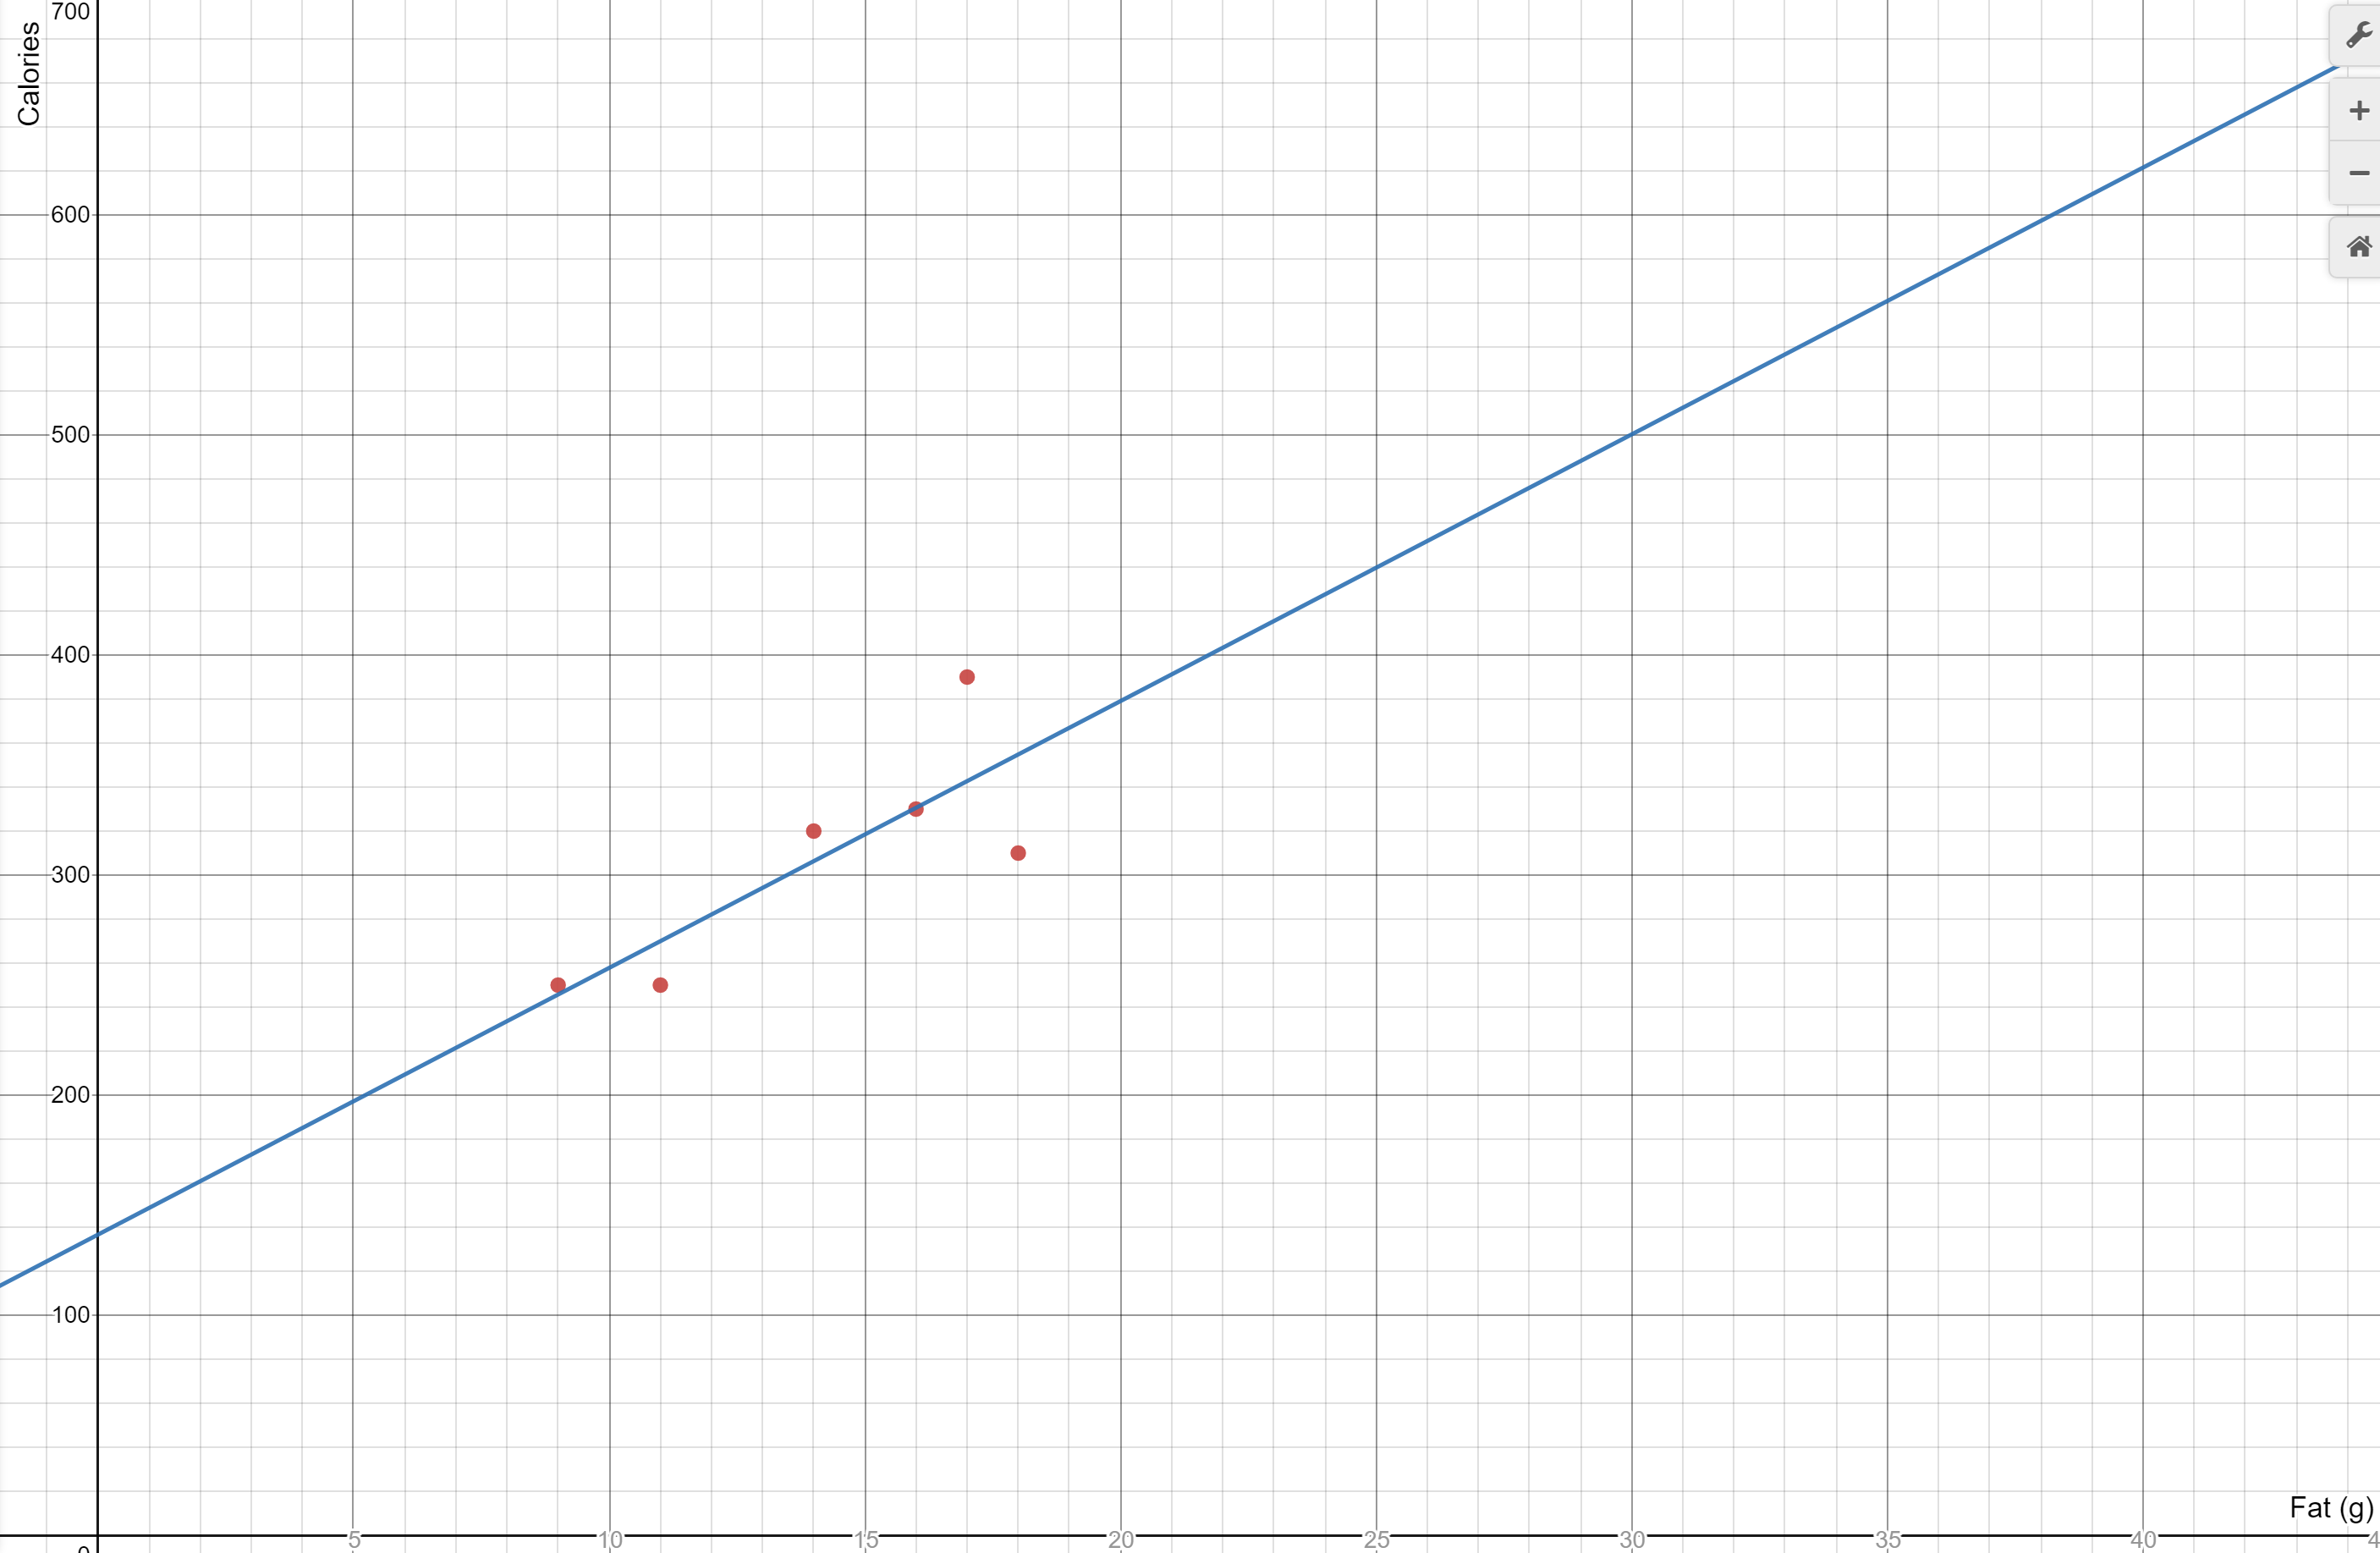
\includegraphics[width=4in]{graph2.png}
    \end{center}
}